\vskip -2\baselineskip plus -1fil
\begin{IEEEbiography}
    [{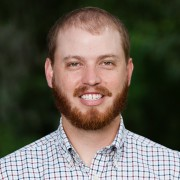
\includegraphics[width=1in,height=1.25in,clip,keepaspectratio]{images/jravan.jpeg}}]{John Ravan}
received his B.S.C.S and M.S.S.E from The Citadel in Charleston, SC in 2011 and 2014. He is currently a student at the University of South Carolina where he is pursuing a PhD in Computer Science. His research interests are in web services, databases, and security. He is also a Senior Software Engineer for Tabula Rasa HealthCare where he currently builds APIs for common medication data transmission. Mr. Ravan also serves as the CTO for Charleston-based non-profit Global Leadership International where he determines the use and procedures for information technology.
\end{IEEEbiography}
\vskip -2\baselineskip plus -1fil
\begin{IEEEbiography}
    [{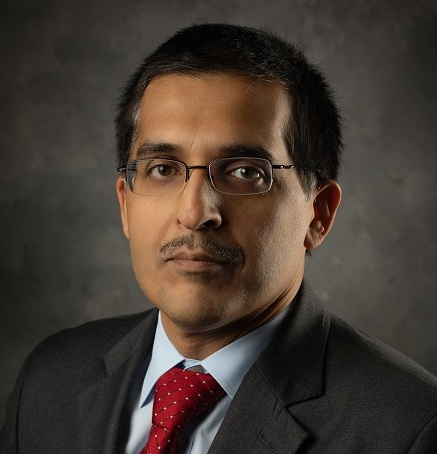
\includegraphics[width=1in,height=1in,clip,keepaspectratio]{images/Banik.jpg}}]{Shankar M. Banik}
received the BTech (Hons) degree in Computer Science and Engineering from the Indian Institute of Technology, Kharagpur, in 1997 and the MS and PhD degrees in Computer Science from the University of Oklahoma in 2001 and 2006, respectively. In 2006, he joined the Department of Mathematics and Computer Science, The Citadel, where he is currently a Professor of Computer science, Graduate Program Director for Computer Science, and Co-director for Citadel Center for Cyber, Intelligence, and Security Studies. His research interests include overlay networks, multicasting, network security, distributed database systems, and graph algorithms. 
\end{IEEEbiography}
\vskip -2\baselineskip plus -1fil
\begin{IEEEbiography}
    [{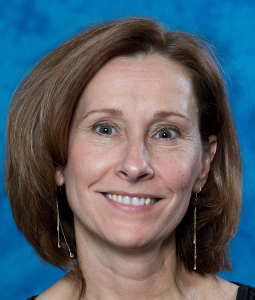
\includegraphics[width=1in,height=1in,clip,keepaspectratio]{images/farkas.jpeg}}]{Csilla Farkas} is a Professor in the Department of Computer Science and Engineering and Director of the Center for Information Assurance Engineering at the University of South Carolina. Dr. Farkas’ research interests include information security, data inference problem, financial and legal analysis of cyber crime, and security and privacy on the Semantic Web. She is a recipient of the NSF Career award. The topic of her award is “Semantic Web: Interoperation vs. Security – A New Paradigm of Confidentiality Threats.” Csilla Farkas received her PhD from George Mason University. In her dissertation she studied the inference and aggregation problems in multilevel secure relational databases. She received a MS in computer science from George Mason University and BS degrees in computer science and geology from SZAMALK, Hungary and Eotvos Lorand University, Hungary, respectively.
\end{IEEEbiography}
\vskip -2\baselineskip plus -1fil